\documentclass[../main.tex]{subfiles}
\graphicspath{{\subfix{../figures/}}}

\begin{document}
\section{实验步骤}
\subsection{攻击准备}
准备硬件和软件:
\begin{itemize}
  \item 硬件:
    \begin{itemize}
      \item PC.
      \item ESP8266 Wi-Fi 模块.
    \end{itemize}
  \item 软件:
    \begin{itemize}
      \item Arduino IDE.
      \item 安信可串口调试助手.
      \item Flash Download Tool.
      \item esp8266\_deauther.
      \item Python-3.
    \end{itemize}
\end{itemize}

下面编译生成需要在 ESP8266 上执行的固件:
\begin{minted}{sh}
git clone https://github.com/SpacehuhnTech/esp8266_deauther
cd esp8266_deauther/esp8266_deauther
python3 ../utils/arduino-cli-compile.py 2.5.0
\end{minted}

编译完成后会得到一个 bin 文件, 需要将这个文件上传至 ESP8266, 需要用到 Flash
Download Tool(需先将 ESP8266 同 PC 连接).

\begin{figure}[H]
  \begin{center}
    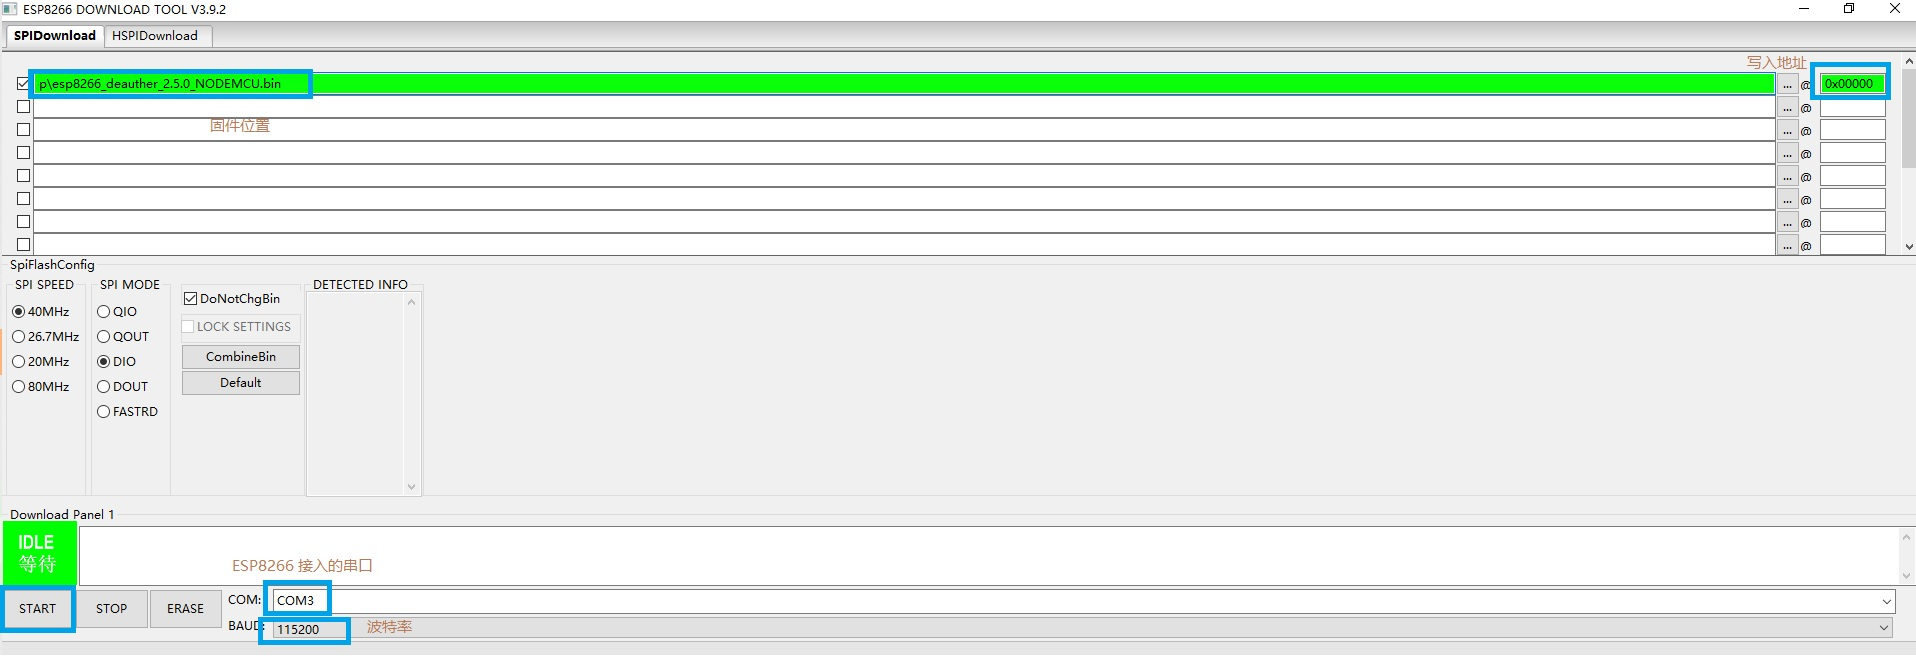
\includegraphics[width=0.30\textwidth]{flash.jpg}
  \end{center}
  \caption{代码烧录}
\end{figure}

设置完毕后点击 ``Start'' 开始烧录.

至此我们完成了环境设置和代码上传, 下面就是``指挥'' ESP8266 实施攻击.
%
\subsection{实施攻击}
首先确保客户端(受害者, Victim)已经连接到 AP:
\begin{figure}[H]
  \begin{center}
    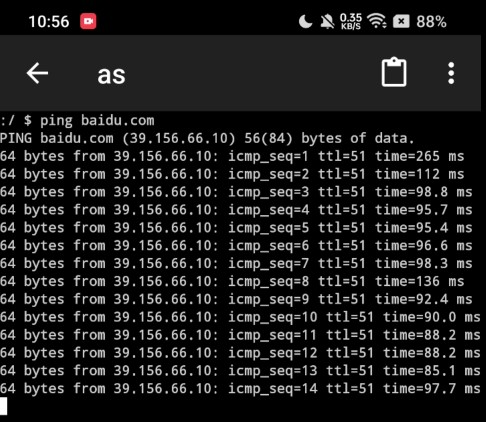
\includegraphics[width=0.30\textwidth]{normal_ping.jpg}
  \end{center}
  \caption{Victim is online.}
\end{figure}

使用安信可串口调试助手扫描附近的通信:
\begin{figure}[H]
  \begin{center}
    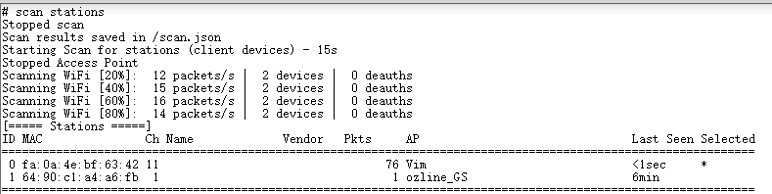
\includegraphics[width=0.40\textwidth]{attacker_scan.jpg}
  \end{center}
  \caption{Attacker scans stations.}
\end{figure}

攻击者选择受害者:
\begin{figure}[H]
  \begin{center}
    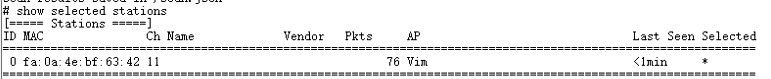
\includegraphics[width=0.40\textwidth]{attacker_select_stations.jpg}
  \end{center}
  \caption{Attacker selects the victim.}
\end{figure}

攻击者实施攻击:
\begin{figure}[H]
  \begin{center}
    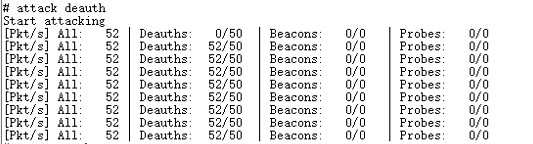
\includegraphics[width=0.40\textwidth]{attacker_attack.jpg}
  \end{center}
  \caption{Attacker starts attacking.}
\end{figure}

受害者下线:
\begin{figure}[H]
  \begin{center}
    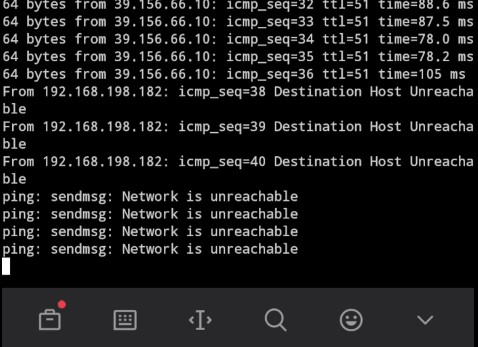
\includegraphics[width=0.30\textwidth]{abnormal_ping.jpg}
  \end{center}
  \caption{Victim is offline.}
\end{figure}
%
\end{document}
